\documentclass[11pt,a4paper]{article}
\usepackage[T1]{fontenc}\usepackage[utf8]{inputenc}
\usepackage{lmodern,microtype,amsmath,amssymb,amsthm,mathtools}
\usepackage{booktabs,longtable,array,enumitem,xcolor,geometry,fancyhdr,hyperref,graphicx}
\geometry{margin=22mm}
\hypersetup{colorlinks=true,linkcolor=blue!55!black,urlcolor=blue,citecolor=blue!55!black,
 pdftitle={FIN ST1722--ST1811: Repository-Wide Falsification of the Kernel-to-Ltotal Chain and the Decisive Source-Action Gate},
 pdfauthor={Krzysztof Żuchowski}}
\pagestyle{fancy}\fancyhf{}\fancyhead[L]{FIN ST1722--ST1811}\fancyhead[R]{Release 11.03}\fancyfoot[C]{\thepage}\setlength{\headheight}{14pt}
\newtheorem{theorem}{Theorem}\newcommand{\status}[1]{\textsf{[#1]}}

\begin{document}
\begin{titlepage}\centering\vspace*{13mm}
{\Huge\bfseries FIN ST1722--ST1811\par}\vspace{4mm}
{\LARGE Repository-Wide Falsification of the\par}\vspace{2mm}
{\LARGE Kernel-to-$L_{\rm total}$ Chain\par}\vspace{2mm}
{\Large and the Decisive Source--Action Gate\par}\vspace{11mm}
{\Large Krzysztof \.Zuchowski\par}
{\normalsize Independent Researcher --- Fractal Information Theory Project\par}
{\normalsize ORCID: 0009-0002-0909-3613\par}\vspace{9mm}
{\large Six adaptive research rounds --- 90 programmes\par}
{\large Release 11.03 --- 31 August 2026\par}
\vfill
\begin{minipage}{.88\textwidth}\small
This report audits the current FIN repository state, with particular attention
to \texttt{STRICT\_KERNEL\_LAGRANGIAN\_AND\_EOM\_DRAFT.md},
\texttt{STRICT\_EQUATION\_SHEET\_KERNEL\_TO\_LTOTAL\_CURRENT.md}, the
strict/legacy split, APD completion, current no-go maps, and all recent strict
and operational results.  Its purpose is falsification, not confirmation.
\end{minipage}\vfill
{\small English mathematical referee-style research report.}
\end{titlepage}

\begin{abstract}
ST1722--ST1811 perform an adversarial reconstruction of the current FIN route
from legacy and strict kernels to effective moments, couplings, a displayed
$L_{\rm total}$ and covariant equations of motion.  The principal conclusion
is negative but structurally decisive: the current chain is not a derivation
of a unique gauge-covariant physical action.

First, the APD completion factor is analysed as a mathematical object.  On the
finite integer $Z_{12}$ distance carrier, the legacy kernel is nonzero and the
diagonal multiplier $Q_i=K_{\rm strict}(i)/K_{\rm legacy}(i)$ exists uniquely.
But this is automatic for every nonzero input vector and arbitrary target.
The multiplier has six positive and six negative values, so it is not a
positive channel.  In the real continuum the legacy cosine vanishes at
$d=4/3+4k$, while the strict target is nonzero at the first such points.
Therefore the APD ratio has nonremovable poles and no bounded continuous global
multiplicative completion exists.  P2363 remains correct only as a finite-
domain and local-germ moment identity; it is not an independently sourced
global bridge.

Second, literal variation of the displayed action reveals internal defects.
The term $-y\phi\bar\psi\psi$ produces $+y\bar\psi\psi$ in the scalar Euler row
under the equation sheet's convention, whereas the compact draft displays the
opposite sign.  The interaction $A_\mu A^\mu\phi^2$ is not locally gauge
invariant by itself and violates the off-shell Ward identity.  A gauge repair
requires a complex charged scalar with both derivative current and seagull
terms tied to one charge, or an additional Higgs/Stueckelberg field.  A Proca
interpretation is possible only by abandoning the gauge/BRST claim.  Moreover,
the displayed covariant EOM rows contain Higgs, cubic, $RF^2$ and curvature-
squared terms absent from the displayed action, while omitting explicit rows
from its $A^2\phi^2$ interaction.  No single literal displayed action generates
all current covariant rows.

Third, the three-moment map at $d_{\rm ref}=1$ is neither reference invariant
nor identifying.  Its Jacobian with respect to $(\omega,\phi,\beta,\eta)$ has
rank three, and distinct parameter tuples are constructed with the same
$(c_0,c_1,c_2)$ to numerical residuals near $10^{-12}$ but different kernel
values away from the reference point.  The effective multipliers change
substantially when $d_{\rm ref}$ is moved, and five free base couplings absorb
arbitrary effective targets wherever the factors are nonzero.  A fourth jet
locally restores parameter rank, but not physical scales or a source law.

Fourth, the finite strict kernel matrix $W$ is tested as a propagator.  In the
current construction $W=sI-A$.  It cannot equal a normal-ordered resolvent
$a(A+m^2I)^{-1}-cI$ on seven distinct eigenvalues.  Its spectrum has seven
negative and five positive modes, so using $W$ as a Euclidean covariance gives
an indefinite inverse Hessian.  The unavoidable variational object is instead
the positive Dirichlet action
\[
S_A[f;J]=\frac12f^TAf-J^Tf,
\]
whose Green operator is $A^+$ on the mean-zero subspace.  This action unifies
finite Green response, heat, unitary and wave functional calculi but does not
select a physical channel, state category, scale or spacetime interpretation.

The current FIN mathematics therefore survives as a finite Dirichlet--Markov--
spectral information geometry with conditional operational models.  It is not
currently a fundamental physical theory.  The highest-value next theorem is
to derive or refute one globally regular, refinement-compatible,
gauge-covariant source action directly from strict algebra/Dirichlet data,
with every EOM regenerated by literal variation.  A seven-row decisive gate is
provided; the current strict repository passes zero complete rows.
\end{abstract}

\tableofcontents\newpage

\section{Repository scope and method}

The audit uses the current project guardrails, strict/legacy split notes,
strategic state maps, the two requested Lagrangian/EOM documents, P1866,
P2316, P2362--P2366, the P2685--P2687 reverse-closure no-go sequence, the
P3140--P3172 unit/selector state map, and Releases 10.89--11.02.  The existing
negative results are treated as established unless a stronger direct
calculation changes their scope.

The six adaptive rounds were not precommitted.  Each round selected the next
object from the strongest defect found in the previous one:
\[
\text{action/EOM audit}	o\text{APD}	o\text{literal variation}	o
\text{moment map}	o\text{propagator/action}	o\text{decisive gate}.
\]

\section{Round I: ST1722--ST1736 --- action/EOM type audit}

The displayed covariant action contains, schematically,
\[
\{(\nabla\phi)^2,\phi^2,\phi^4,\phi^2R,
\bar\psi iD\psi,\phi\bar\psi\psi,F^2,A^2\phi^2,R,\Lambda\}.
\]
The later covariant EOM rows additionally contain a separate $H$ field,
$\lambda_3\phi^2$, $\phi^2H^\dagger H$, $RH$, $RF^2$, curvature-squared
tensors and a full $T_{\mu\nu}^{\rm SM+mix}$.  Those rows require additional
action terms and field definitions; they cannot be generated by renaming the
coefficients in the displayed scaffold.

Conversely, the later covariant $E_\phi$ and $E_A$ rows do not explicitly carry
the pair of terms generated by the displayed $A^2\phi^2$ interaction.  The
compact earlier scalar template does, showing that the two equation lists come
from different lineages rather than one frozen action.

The compact statement also adds ordinary scalar/fermion/gauge Lagrangians to a
gravity \emph{density} already containing $\sqrt{-g}$.  The later covariant
presentation repairs that notation, but it does not repair the mixed term
provenance.

Finally, solving two FRW residual equations algebraically for $H^2$ and
$\Lambda$ and substituting the solution back proves an algebraic normal form.
It does not derive $\rho,p,H,\Lambda$, validate the off-FRW tensor equations or
provide a physical background source.

\section{Round II: ST1737--ST1751 --- APD completion}

\subsection{Finite completion theorem}

Let $L_i\ne0$ on a finite carrier and let $S_i$ be arbitrary.  There is exactly
one diagonal multiplier
\[
Q_i=\frac{S_i}{L_i}
\]
satisfying $Q_iL_i=S_i$.  Thus a zero assembly residual is automatic after the
target appears in the definition of $Q$; it does not identify a mechanism.

The repository correctly proves that the legacy cosine does not vanish on
integer $d=0,\ldots,11$.  The APD values are therefore finite there.  Direct
replay gives six positive and six negative multipliers, so $Q_{\rm APD}$ is not
a positive diagonal measure, Markov channel or completely positive operation.

\subsection{Global obstruction}

For the legacy parameters,
\[
\cos\left(\frac\pi4d+\frac\pi6\right)=0
\quad\Longleftrightarrow\quad
d=\frac43+4k.
\]
At the first three nonnegative zeros the strict kernel equals approximately
\[
0.3423917,quad0.0189960,quad-0.00563505,
\]
and is nonzero.  Therefore $K_{\rm strict}/K_{\rm legacy}$ has nonremovable
poles.

\begin{theorem}[APD global multiplicative no-go]
No finite continuous multiplier on a real domain containing a legacy zero with
nonzero strict target can satisfy
$K_{\rm legacy}Q=K_{\rm strict}$.
\end{theorem}

Around $d_{\rm ref}=1$, the nearest real pole is at $4/3$, so the APD factor is
a valid local analytic germ.  Its moment equality is then a derivative of the
identity used to define the ratio.  This preserves P2363 exactly in its stated
finite nonzero-domain/local-moment scope while forbidding promotion to a global
physical completion operator.

An additive repair
$K_{\rm strict}=K_{\rm legacy}+(K_{\rm strict}-K_{\rm legacy})$ is regular but
imports the complete target difference.  General nonlocal linear maps sending
one finite vector to another are infinitely nonunique.  Neither alternative
supplies a strict source law.

\section{Round III: ST1752--ST1766 --- literal variation and gauge test}

Suppressing only irrelevant tensor notation, the displayed terms contain
\[
L=\frac12(\partial\phi)^2-\frac12m^2\phi^2-\frac\lambda4\phi^4
-y\phi B+\frac g2A^2\phi^2+\xi R\phi^2,
\qquad B=\bar\psi\psi.
\]
Using the equation sheet's convention
$E_\phi=\partial(\partial L/\partial(\partial\phi))-\partial L/\partial\phi$
gives
\[
E_\phi=\Box\phi+m^2\phi+\lambda\phi^3
+yB-gA^2\phi-2\xi R\phi.
\]
The compact draft prints $-yB$.  The relative Yukawa sign therefore disagrees
with literal variation of its own displayed action.

For an Abelian gauge transformation
$A_\mu\mapsto A_\mu+\partial_\mu\alpha$, the infinitesimal variation of the
seagull term is
\[
\delta L=g\phi^2A^\mu\partial_\mu\alpha
=-g\alpha\,\partial_\mu(\phi^2A^\mu)+\text{boundary},
\]
which is not identically zero.  The gauge EOM divergence inherits the same
Ward defect.

A locally invariant scalar repair requires a complex charged field:
\[
|D\Phi|^2=|\partial\Phi|^2
+iqA_\mu(\Phi^*\partial^\mu\Phi-\Phi\partial^\mu\Phi^*)
+q^2A^2|\Phi|^2.
\]
The derivative current and seagull are mandatory and share the coefficient
$q$.  The current draft has the seagull with independent $g_{\rm eff}$ and no
corresponding derivative current.  Alternatively $A$ may be read as a Proca
field, but then local gauge/BRST language must be dropped or a Stueckelberg/
Higgs field added.

The quartic normalization also differs: $-\lambda\phi^4/4$ yields
$\lambda\phi^3$, while the sector row $\lambda_4\phi^3/3!$ corresponds to a
$\lambda_4\phi^4/4!$ convention.  No map is exported, and the cubic term is
absent from the displayed action.

\begin{theorem}[single displayed action no-go]
The current displayed $L_{\rm total}$ does not generate all current covariant
EOM rows and is not a local gauge-invariant action in the declared field
content.
\end{theorem}

Reduced termwise models with zero recomposition residual remain internally
valid as separate reduced actions.  They do not prove the global claim.

\section{Round IV: ST1767--ST1781 --- moment-map falsification}

The moment feature map is
\[
(\omega,\phi,\beta,\eta;d_{\rm ref})
\longmapsto(c_0,c_1,c_2).
\]
For the same strict kernel, moving $d_{\rm ref}$ from $0.5$ to $1$ to $2$
changes the mass/$\xi$ multiplier $1+c_0$ from approximately
$1.75170$ to $1.46999$ to $1.19204$.  The $g$ multiplier $1+c_2$ changes from
$1.01823$ to $1.23191$ to $1.07847$.  No canonical reference length is
exported.

Under $d'=ad$, the derivatives transform as
\[
c'_0(1)=K(1/a),\quad
c'_1(1)=a^{-1}K'(1/a),\quad
c'_2(1)=\frac12a^{-2}K''(1/a).
\]
Thus the map is not coordinate-scale invariant.

At the nominal tuple, the $3\times4$ Jacobian has singular values
\[
0.39633,quad0.28037,quad0.09566
\]
and rank three.  A local null direction exists.  Fixing $\eta$ to $1.79$,
$1.81$ and $1.85$, numerical root solves produce distinct
$(\omega,\phi,\beta)$ tuples with the same three moments to residuals between
$10^{-15}$ and $10^{-12}$, while their kernel values differ away from the
reference point.

The five maps
\[
m^2_{\rm eff}=m^2(1+c_0),\quad
\lambda_{\rm eff}=\lambda(1+c_1^2),\quad\ldots
\]
retain five free base couplings.  Wherever the factors are nonzero, any target
effective coupling is obtained by dividing it by the factor.  The map therefore
does not predict absolute couplings.  Squaring $c_1$ additionally deletes its
sign.

A fourth normalized derivative raises the local parameter Jacobian to rank
four with condition number about $10.8$.  This is a constructive mathematical
repair of local parameter identifiability, not a physical source or scale.

\section{Round V: ST1782--ST1796 --- canonical action and propagator test}

The strict finite generator defines the unavoidable Dirichlet action
\[
S_A[f;J]=\frac12f^TAf-J^Tf.
\]
Its variation is $Af=J$.  Since $A\mathbf1=0$, a solution requires
$\mathbf1^TJ=0$ and is unique only modulo $f\mapsto f+c\mathbf1$.  On the
mean-zero space the Green operator is the Moore--Penrose inverse $A^+$.
Adding $m^2>0$ gives the positive family
\[
G_m=(A+m^2I)^{-1},
\]
but $m$ is extra input.

In the frozen FIN matrix construction,
\[
W=sI-A,qquad s=1.660307278766099.
\]
Suppose, even after normal-order subtraction, that
\[
s-\lambda=\frac a{\lambda+m^2}-c
\]
on the spectrum of $A$.  Multiplication by $\lambda+m^2$ gives a nonconstant
quadratic polynomial that cannot be constant at more than two distinct
$\lambda$ values.  The strict $A$ has seven distinct eigenvalues.

\begin{theorem}[same-generator propagator obstruction]
No constants $a,m^2,c$ make the current $W$ a normal-ordered resolvent of the
same $A$ on its full spectrum.
\end{theorem}

Numerically, $W$ has seven negative and five positive eigenvalues.  It is
invertible, but an action whose Euclidean covariance is $W$ has Hessian
$W^{-1}$ and is unbounded below.  Therefore $W$ is currently an adjacency/
coupling matrix, not the positive Green covariance of the canonical $A$
action.  It could be a propagator of a different parent operator only if that
operator and its stability structure are independently supplied.

The same $A$ still generates heat, unitary and wave calculi.  The Dirichlet
action does not select which is physical.  A noncommutative spectral action
would additionally need an algebra, representation, Dirac grading/reality,
cutoff function and dimensional cutoff.

\begin{figure}[ht]
\centering
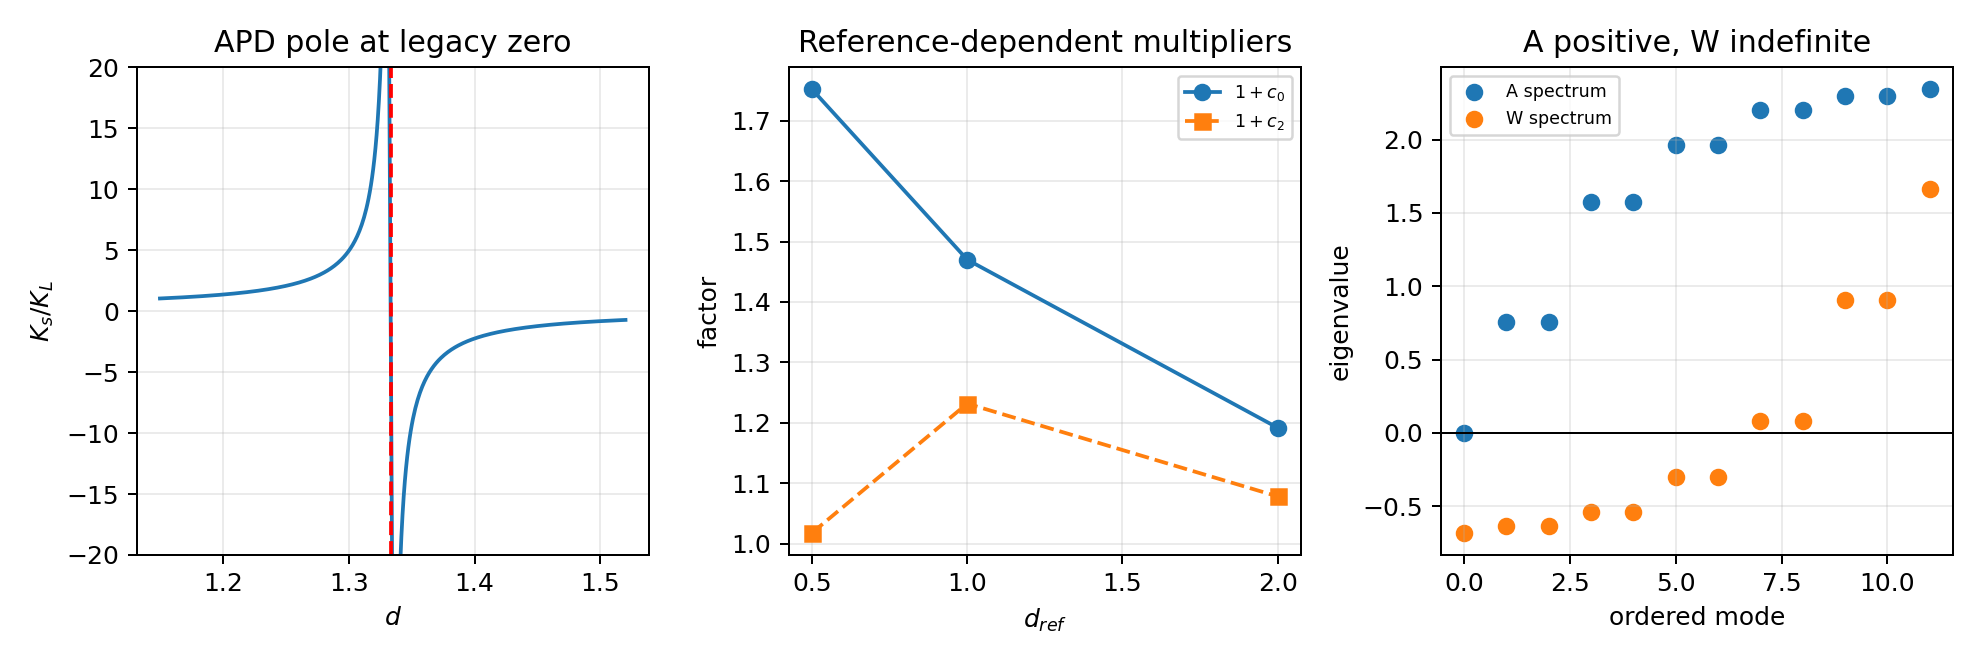
\includegraphics[width=.98\textwidth]{FIN_ST1722_ST1811_Figures/repository_falsification_summary.png}
\caption{Left: the first nonremovable APD pole.  Centre: reference dependence
of selected coupling multipliers.  Right: positive $A$ spectrum versus
indefinite $W$ spectrum.}
\end{figure}

\section{Round VI: ST1797--ST1811 --- decisive verdict}

\subsection{What is proved, refuted and conditional}

\begin{longtable}{@{}p{.34\textwidth}p{.20\textwidth}p{.36\textwidth}@{}}
\toprule
Object/claim & Status & Boundary \\
\midrule\endhead
finite APD ratio on $Z_{12}$ & \status{Proven} & automatic diagonal completion \\
global bounded/positive APD & \status{Refuted} & nonremovable poles/signs \\
P2363 local moment identity & \status{Proven local} & finite nonzero domain/germ \\
one displayed covariant action for all EOM & \status{Refuted} & term/sign/gauge defects \\
reduced/FRW normal forms & \status{Conditional} & named actions/backgrounds \\
three moments identify strict kernel & \status{Refuted} & rank-three four-parameter map \\
moment map predicts couplings & \status{Refuted} & free bases/reference choice \\
$W$ is Green of same $A$ & \status{Refuted} & spectral polynomial obstruction \\
finite Dirichlet form of $A$ & \status{Proven} & dimensionless finite model \\
OA dual-dynamics protocols & \status{Conditional/certified} & selected state/channel/apparatus model \\
fundamental physical theory & \status{Not established} & decisive source-action rows absent \\
\bottomrule
\end{longtable}

\subsection{The decisive source--action gate}

A future claim connecting FIN to unique physics must jointly supply:
\begin{enumerate}[label=G\arabic*.]
\item a globally regular, non-tautological strict source map;
\item canonical refinement/continuum geometry and dimensional scale;
\item one typed gauge/diffeomorphism-consistent action;
\item literal variation regenerating every claimed EOM with residual tables;
\item state, channel, clock, preparation, instrument and record;
\item parameter values or sharp predictions not absorbable into free bases;
\item a held-out physical forward model and falsifiable record.
\end{enumerate}

Removing any row reproduces a known countermodel: APD quotient tautology,
reference/unit torsors, gauge--Proca ambiguity, mixed-lineage EOM, A-only state
nonuniqueness, free-coupling absorption or absence of physics evidence.  The
current strict repository has useful subcomponents, but zero complete rows
passing all obligations of their class.

\subsection{Route ranking}

\begin{longtable}{@{}p{.53\textwidth}p{.18\textwidth}p{.18\textwidth}@{}}
\toprule
Route & Rigorous-success estimate & Physics decision power \\
\midrule\endhead
publish finite Dirichlet/Markov/spectral FIN mathematics & 0.90 & 0.25 \\
derive refinement-compatible continuum Dirichlet form, scale and causal observable & 0.35 & 0.80 \\
derive gauge-covariant spectral/source action from independently sourced algebra & 0.18 & 1.00 \\
repair current APD--three-moment--$L_{\rm total}$ chain & 0.03 & 0.70 \\
conditional OA laboratory discrimination & 0.45 & 0.55 \\
\bottomrule
\end{longtable}

These are strategic judgments, not probabilities derived from data.

\section{Most important result and highest-value next direction}

The most important result is the conjunction of independent obstructions:
\[
\boxed{
\text{current APD}\to\text{three moments}\to\text{free couplings}
\to L_{\rm total}
\text{ is not a derivation of unique physics}.}
\]
No single defect alone establishes this.  The conclusion survives attempts to
reinterpret APD locally, repair gauge invariance, move the reference point,
add a fourth moment and reinterpret $W$ as a propagator.

The deepest object surviving every falsification attempt is
\[
\boxed{
\text{a finite Dirichlet--Markov--spectral information geometry}
}
\]
together with exact contextual reductions and conditional operational channel
models.  It is mathematically coherent and potentially publishable, but it is
not yet fundamental physics.

The single highest-value next theorem is:
\begin{quote}
\emph{derive or refute a globally regular, refinement-compatible,
gauge-covariant source action directly from strict algebra/Dirichlet data, and
regenerate every field equation by literal variation before fitting any
Standard-Model or gravitational coefficient.}
\end{quote}

The immediate falsification order is global regularity, Ward/gauge identity,
Euler regeneration, refinement naturality, scale covariance and a
nonabsorbable prediction.  Failure at any row should stop the route.  Repeating
APD quotients, three-moment coupling maps or additional receiver-level SM/GR
rows cannot resolve the established obstructions.

\section{Final interpretation}

\begin{quote}
FIN is presently a rigorous finite spectral-information and Dirichlet/Markov
framework with unusually strong internal no-go discipline and increasingly
precise conditional operational tests.  The current repository does not
derive a globally regular bridge, a unique gauge-covariant action, physical
units, state semantics or experimental law from the kernel.  It therefore
cannot presently be classified as a fundamental physical theory.  Its most
scientifically valuable next step is a single source--action theorem (or its
no-go), not another phenomenological completion of the existing scaffold.
\end{quote}

\appendix
\section{Six-round ledger}
\begin{longtable}{@{}p{.18\textwidth}p{.34\textwidth}p{.38\textwidth}@{}}
\toprule
Range & Target & Verdict \\
\midrule\endhead
ST1722--ST1736 & repository action/EOM map & mixed lineage and gauge defects \\
ST1737--ST1751 & APD completion & finite/local valid; global physical no-go \\
ST1752--ST1766 & literal variation & Yukawa sign, gauge and source mismatch \\
ST1767--ST1781 & moment-to-coupling map & reference/rank/prediction no-go \\
ST1782--ST1796 & canonical action/propagator & Dirichlet survives; $W$-Green refuted \\
ST1797--ST1811 & synthesis & decisive seven-row source--action gate \\
\bottomrule
\end{longtable}

\section{Reproducibility}
The authoritative result sets run from
\path{FIN_ST1722_ST1736_Results.json} through
\path{FIN_ST1797_ST1811_Results.json}.  Each contains fifteen programmes and
packet SHA-256 references.  The combined test
\path{test_fin_st1722_st1811.py} verifies all ninety packets, APD poles/signs,
literal variation, moment rank, propagator spectrum, decisive gate, figure and
nonpromotion boundaries.

\section{Nonclaims}
This report does not prove that no future FIN extension can become physical.
It does not invalidate the finite strict kernel, Dirichlet form, spectral
theorems, reduced actions or conditional OA tests in their stated scopes.  It
does not complete legacy role transfer, QW-2191, units, Standard Model,
gravity, $L_{\rm total}$ or Theory of Everything.  All future FIN PDFs remain
English.

\begin{thebibliography}{9}
\bibitem{reed} M. Reed and B. Simon, \emph{Methods of Modern Mathematical Physics I}, Academic Press.
\bibitem{peskin} M. Peskin and D. Schroeder, \emph{An Introduction to Quantum Field Theory}, Addison--Wesley.
\bibitem{connes} A. Connes and M. Marcolli, \emph{Noncommutative Geometry, Quantum Fields and Motives}, AMS.
\end{thebibliography}
\end{document}
